%%
% Copyright (c) 2017 Saúl Piña <sauljabin@gmail.com>.
%
% This program is free software: you can redistribute it and/or modify
% it under the terms of the GNU General Public License as published by
% the Free Software Foundation, either version 3 of the License, or
% (at your option) any later version.
%
% This program is distributed in the hope that it will be useful,
% but WITHOUT ANY WARRANTY; without even the implied warranty of
% MERCHANTABILITY or FITNESS FOR A PARTICULAR PURPOSE.  See the
% GNU General Public License for more details.
%
% You should have received a copy of the GNU General Public License
% along with this program.  If not, see <http://www.gnu.org/licenses/>.
%%

\capitulo{Diseño e Ingeniería de la Propuesta}

En este capítulo se describen los aspectos relacionados a la implementación
del modelo afectivo de MASOES propuesto por \cite{perozo2011}.

En primer lugar, se explican los aspectos arquitecturales de la implementación,
relevantes para entender el funcionamiento de la plataforma.
En segundo lugar, se exponen a nivel de implementación los componentes individuales y
colectivos de los agentes emocionales, descritos a nivel de diseño por \cite{perozo2011}.
Por último, se detalla lo referente a la herramienta computacional desarrollada.

\seccion{Aspectos Arquitecturales de la Propuesta}

Como paradigma de software para el desarrollo de la implementación,
se seleccionó la Programación Orientada a Agentes (POA). Este paradigma propuesto
por \cite{shoham1993agent}, esencialmente modela una aplicación como una
colección de componentes llamados agentes \citep{bellifemine2007developing}.
Permite llevar a cabo la materialización a nivel de aplicación de los sistemas
multiagente.
La POA y la Programación Orientada a Objetos (POO) son
compatibles, la primera puede ser vista como una especialización de la segunda \citep{shoham1993agent},
además, dependiendo del lenguaje de programación pueden mezclarse.

Por otra parte, se usó JADE \eningles{Java Agent
DEvelopment}, uno de los marcos de trabajo con paradigma de POA
más populares, implementado en el lenguaje de programación Java.
JADE provee bibliotecas de clases para la creación de agentes mediante
la herencia y la sobrescritura de comportamientos. Incluye
un conjunto de herramientas gráficas para la monitorización y administración de los agentes.
Además de ser un marco de trabajo, JADE se considera una plataforma,
debido a que contiene un entorno en el que los agentes se ejecutan
y se controla su ciclo de vida. Una de las característica más importante de JADE
es que cumple con las especificaciones estándar FIPA \eningles{Foundation for Intelligent Physical Agents},
las cuales representan una colección de normas que tienen como objetivo promover la interoperabilidad
de agentes heterogéneos y los servicios que pueden representar. La \refilustracion{arquitectura-propuesta}
muestra la arquitectura de la plataforma JADE.

\begin{ilustracion}[fuente=\yo, etiqueta=arquitectura-propuesta, titulo={Arquitectura de JADE Conjuntamente con MASOES}]
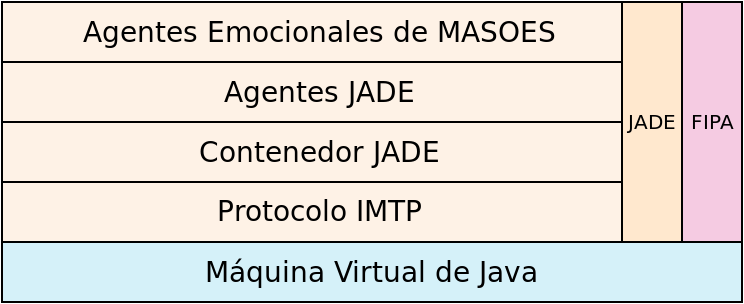
\includegraphics[width=8cm]{ilustraciones/propuesta/arquitectura.png}
\end{ilustracion}

La capa que conforma la base de la
arquitectura es la maquina virtual de Java y es la que permite
instanciar la plataforma, sobre ella se encuentra Jade, compuesta a su vez
por:

\textbf{Protocolo IMTP} \eningles{Instant Message Transfer Protocol}.
Protocolo utilizado por los agentes
para comunicarse entre sí localmente o en una red de computadores,
a través de mensajes estandarizados por FIPA \refpilustracion{comunicacion-entre-hosts}.

\textbf{Contenedor JADE}. Proporciona
todos los servicios necesarios para alojar y ejecutar agentes.

\textbf{Agentes JADE}. Son entidades de software que poseen proceso propio, comportamiento,
ciclo de vida y son capaces de recibir y enviar mensajes.

La capa superior corresponde a la implementación de los agentes emocionales
propuestos para MASOES. Dicha capa funciona como una extensión del marco de trabajo
de JADE. Proporciona un agente emocional que contiene la implementación
del componente conductual y el modelo afectivo de MASOES.

\begin{ilustracion}[fuente=\yo, etiqueta=comunicacion-entre-hosts, titulo={Comunicación Entre Agentes de JADE}]
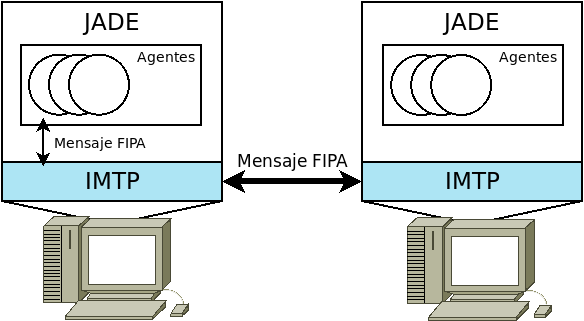
\includegraphics[width=8cm]{ilustraciones/propuesta/comunicacion-entre-hosts.png}
\end{ilustracion}

Cuando se inicia el contenedor principal, dos agentes especiales son automáticamente
instanciados por JADE, cuyos roles están definidos por FIPA y utilizan
la especificación \comillas{FIPA Agent Management} para la comunicación a través de mensajes
\citep{fipaAgentManagement}:

\textbf{Agente AMS} \eningles{Agent Management System}. El AMS  controla la plataforma.
Es el único que puede crear y destruir a otros agentes, destruir contenedores y detener la plataforma.
Se encarga de asignarle un código a cada agente, y posee el servicio de páginas blancas, es decir,
un registro de todos los agentes. Cuando un agente desea conocer la existencia de otro
en el entorno, se comunica con el AMS.

\textbf{Agente DF} \eningles{Directory Facilitator}. El DF proporciona un directorio que
anuncia los servicios disponibles en la plataforma.
Un agente dentro del
entorno puede notificarle al agente DF cual es su rol y publicar
sus servicios (acciones), dándose a conocer a otros.

\seccion{Aspectos Propuestos a Nivel Individual}

\label{propuesta-nivel-individual}

En esta sección se describe una propuesta de ontología para MASOES
y la implementación interna de los agentes emocionales.
Además, se explica como ocurre el proceso de comunicación entre los agentes.

\subseccion{Propuesta de Una Ontología Para MASOES}

\label{propuesta-ontologia}

JADE requiere para la comunicación entre los agentes, la definición de una ontología.
En JADE una ontología es la definición de los conceptos y relaciones entre ellos, que forman parte
del conocimiento de un agente o una sociedad de agentes. Tanto el emisor como el receptor deben atribuir el
mismo significado a estos elementos para que la comunicación sea efectiva \citep{bellifemine2007developing}.

La necesidad de utilizar ontologías viene dada por la complejidad inherente a
las aplicaciones desarrolladas en el contexto de los sistemas multiagente, haciendo
que se presenten las siguientes dificultades: abundancia de comunicación
entre agentes, interoperabilidad de sistemas y plataformas, y problemas
semánticos.

JADE incorpora funcionalidades para codificar y decodificar las ontologías,
utilizando las especificaciones FIPA \citep{fipaOntology, fipaLanguage}.
Para construir una ontología se debe definir los siguientes elementos:

\begin{vinetas}
    \item \textit{Acciones:} son actividades que pueden llevar a cabo los agentes.
    \item \textit{Conceptos:} representan las entidades que forman parte de la ontología.
    \item \textit{Predicados:} son expresiones que relacionan los conceptos. Son
    necesarios porque en un mensaje nunca se podrá enviar directamente conceptos, solo
    predicados o acciones, los conceptos estarían encapsulados por estos dos últimos.
\end{vinetas}

Los elementos anteriormente expuestos, son proporcionados por JADE en forma de abstracciones,
de manera que puedan ser extendidas para definir una ontología de manera personalizada.
Los predicados deben heredar de \textit{Predicate},
así mismo los conceptos de \textit{Concept} y las acciones de \textit{AgentAction}. Además,
este marco de trabajo provee la clase \textit{AID} que representa el identificador único del agente,
que debe ser utilizado para asignar un emisor y receptor de un mensaje, también puede ser incluido en las
ontologías para representar a un agente.

En este trabajo se define la ontología
\comillas{\codigoenlinea{masoes}} para la
comunicación entre agentes emocionles. Dicha ontología se centra en
poder expresar dos acciones clave: evaluar un estímulo
y consultar el estado emocional.

En la \refilustracion{ontologia-masoes-estimulo} se observa las entidades que conforman la
acción evaluar estímulos.
Para solicitarle a un agente que evalúe un estímulo se le debe enviar
 una acción \textit{EvaluarEstimulo},
internamente esta contiene el concepto \textit{Estimulo} que puede ser de tres tipos,
\textit{Objeto, Accion o Evento}.
El agente en cuestión responderá con un predicado de tipo \textit{EstadoDeAgente},
el cual encapsula los conceptos \textit{EstadoDeEmocion}
y \textit{EstadoDeComportamiento}, y representa el nuevo estado emocional del agente
luego de evaluar el estímulo.
Para apreciar de mejor manera el flujo de comunicación se incluye la \refilustracion{flujo-agente-evaluar-estimulo}.

\begin{ilustracion}[fuente=\yo, etiqueta=ontologia-masoes-estimulo, titulo={Ontología para MASOES, Acción Evaluar Estímulo}]
\includegraphics[width=11cm]{ilustraciones/diagramas-puml/ontologia-masoes-estimulo.png}
\end{ilustracion}

\begin{ilustracion}[fuente=\yo, etiqueta=flujo-agente-evaluar-estimulo, titulo={Flujo de Comunicación, Acción Evaluar Estímulo}]
\includegraphics[width=11cm]{ilustraciones/diagramas-puml/flujo-agente-evaluar-estimulo.png}
\end{ilustracion}

Con respecto a la acción consultar estado emocional se tiene el diagrama de la \refilustracion{ontologia-masoes-estado}.
Es posible conocer el estado emocional de un agente enviando la acción \textit{ConsultarEstadoEmocional},
a diferencia de la acción anterior, esta no tiene ningún concepto. El agente receptor responderá
con un predicado de tipo \textit{EstadoDeAgente} y no modificará su estado emocional actual.
El flujo de comunicación se puede ver en la \refilustracion{flujo-agente-estado}.

\begin{ilustracion}[fuente=\yo, etiqueta=ontologia-masoes-estado, titulo={Ontología para MASOES, Acción Consultar Estado del Agente}]
\includegraphics[width=11cm]{ilustraciones/diagramas-puml/ontologia-masoes-estado.png}
\end{ilustracion}

\begin{ilustracion}[fuente=\yo, etiqueta=flujo-agente-estado, titulo={Flujo de Comunicación, Acción Consultar Estado del Agente}]
\includegraphics[width=8cm]{ilustraciones/diagramas-puml/flujo-agente-estado.png}
\end{ilustracion}

\subseccion{Comunicación Entre Agentes}

Los elementos más importantes en la comunicación entre agentes son:

\textbf{Acto comunicativo} o \textbf{performativa}. Definido en \cite{fipaCommnicativeAct},
se refiere al acto de comunicar en un determinado momento una acción.

\textbf{Lenguaje}. Se utilizó el lenguaje \comillas{\codigoenlinea{fipa-sl}}
\eningles{FIPA Semantic Language (SL)}, es un lenguaje estandarizado en \cite{fipaLanguage}, entendible por el humano,
ya que utiliza una codificación en texto plano.

\textbf{Protocolo}. La especificación FIPA declara diferentes protocolos para
distintas acciones o situaciones. Para el desarrollo de este trabajo se utilizó
el protocolo \comillas{\codigoenlinea{fipa-request}} definido en
\cite{fipaProtocol}. Este protocolo dicta el procedimiento que deben seguir los
agentes al recibir un mensaje y que performativas deben ser usadas para cada
acción. En la \refilustracion{flujo-fipa-protocolo-request}, se aprecia el
diagrama de secuencia de las interacciones entre el emisor y el receptor.
El emisor envía una petición al receptor (performativa
\comillas{\codigoenlinea{request}}), luego el receptor puede aceptar
(performativa \comillas{\codigoenlinea{agree}}) o rechazar la petición
(performativa \comillas{\codigoenlinea{refuse}}). En caso que el agente acepte
la petición, enviará al emisor una respuesta afirmativa (performativa
\comillas{\codigoenlinea{inform}}) si la acción se ejecutó correctamente o
fallida (performativa \comillas{\codigoenlinea{failure}}) si ocurrió un error.

\begin{ilustracion}[fuente=\cite{fipaProtocol}, etiqueta=flujo-fipa-protocolo-request, titulo={Protocolo de Petición FIPA}]
\includegraphics[width=6cm]{ilustraciones/diagramas-puml/flujo-fipa-protocolo-request.png}
\end{ilustracion}

\textbf{Ontología}. Es la definición de los conceptos y relaciones entre ellos, que forman parte
del conocimiento de un agente o una sociedad de agentes. Una ontología
es esencial para lograr una comunicación efectiva en un grupo de agentes.
Los elementos que componen una ontología de JADE (Conceptos, Acciones y Predicados) juegan
diferentes papeles en la comunicación. Como se muestra en la \refilustracion{flujo-fipa-protocolo-ontologia},
el contenido que envía un agente emisor es de tipo \textit{AgentAction} y recibirá
como respuesta un contenido de tipo \textit{Predicate}. Los elementos de tipo \textit{Concept}
pueden ser utilizados tanto por las acciones como por los predicados, para transmitir
una información.

\begin{ilustracion}[fuente=\yo, etiqueta=flujo-fipa-protocolo-ontologia, titulo={Comunicación Entre Emisor y Receptor Usando Ontologías}]
\includegraphics[width=10cm]{ilustraciones/diagramas-puml/flujo-fipa-protocolo-ontologia.png}
\end{ilustracion}

\textbf{Mensaje ACL} \eningles{Agent Communication Language}. Es una estructura
común de transporte de información propuesta por \cite{fipaACL},
es implementada por JADE. En la \refcuadro{parametros-mensajes-acl}, se listan los parámetros
utilizados en la implementación para la comunicación entre agentes emocionales, deben ser
provistos en un mensaje para que la comunicación se logre efectuar.

\begin{cuadro}[etiqueta=parametros-mensajes-acl, titulo={Parámetros de Mensajes ACL Usados en la Implementación}]{l|l}
\toprule
 Parámetro & Descripción \\
\midrule
performative & Acto comunicativo \\
sender & Emisor \\
receiver & Receptor \\
content & Contenido del mensaje \\
conversation-id & Identificación única de la conversación \\
language & Lenguaje de codificación del contenido (\codigoenlinea{fipa-sl}) \\
ontology & Ontología del contenido (\codigoenlinea{masoes}) \\
protocol & Protocolo que rige la comunicación (\codigoenlinea{fipa-request}) \\
\bottomrule
\fuentecuadro{2}{\yo}
\end{cuadro}

\subseccion{Diseño de la Implementación a Nivel Individual}

El diseño a nivel individual de la propuesta abarca las entidades
vinculadas al agente emocional, y que permiten responder
a las solicitudes de otros agentes a través de acciones.
La implementación se llevó a cabo de manera que pueda ser extendida o mejorada,
y para ser utilizada en sistemas multiagente con diferentes dominios.
Uno de los aspectos relevantes de la implementación es que es no limitativa,
en otras palabras, los agentes emocionales pueden comunicarse con cualquier otro agente no emocional
o heterogéneo localmente o a través de una red de computadores e interactuar con ellos.
Por otra parte, la implementación permite que el procesamiento de un estímulo por un agente
pueda hacerse de manera individual, invocando su propio componente conductual, o
recibiendo un estímulo desde otros agentes o el entorno.
En la \refilustracion{diseno-nivel-individual}
se muestra el diseño a nivel individual de la implementación.

\begin{ilustracion}[fuente=\yo, etiqueta=diseno-nivel-individual, titulo={Diseño de la Implementación a Nivel Individual}]
\includegraphics[width=11cm]{ilustraciones/diagramas-puml/diseno-nivel-individual.png}
\end{ilustracion}

A continuación, se definen cada una de las entidades involucradas a
nivel individual:

\textbf{Agent}. Es la clase principal de JADE, todos los tipos de agentes deben
heredar de ella, e incluye otros aspectos relevantes, tales como, el envío y
recepción de mensajes y manejo de comportamientos. Además, posee un hilo de
ejecución propio y está bajo las especificaciones FIPA. Es la unidad básica en
la POA.

\textbf{Behaviour}. Pertenece a JADE, esta clase representa los
comportamientos, acciones, actividades o tareas que puede realizar un agente, debe
ser heredada y sobrescrito su método \textit{action}. Un agente puede
contener uno o muchos comportamientos, y estos, pueden ser detenidos o
reanudados según la necesidad del mismo. Además, pueden ser agregados desde
otros comportamientos, o programados para ser ejecutados en momentos
específicos. Se agregan a través del método \textit{addBehaviour} de la clase
\textit{Agent}. Las implementaciones más usadas (también provistas por JADE) son:
\textit{OneShotBehaviour} (para ejecutar una acción una sola vez),
\textit{CyclicBehaviour} (para un comportamiento repetitivo) y
\textit{FSMBehaviour} (para generar un comportamiento compuesto basado en
máquinas de estado finito).

\textbf{AgenteEmocional}. Es la especialización de
la clase original \textit{Agent} de JADE, desarrollado de manera que contenga
el modelo afectivo de MASOES.
Se debe heredar de este agente en el caso de que se desee construir un agente emocional.

\textbf{ComportamientoResponderEstado}. Esta es
una de la acciones básicas para el agente emocional, se encarga
de responder con la información del estado actual del agente a otro que
la haya solicitado. Este comportamiento se lleva a cabo cuando el
agente emocional recibe una solicitud de acción de tipo \textit{ConsultarEstadoEmocional}.

\textbf{ComportamientoEvaluarEstimulo}. Es la acción más
importante del agente emocional, debido a que es la que recibe un estímulo e
invoca las funciones del componente conductual, modificando el estado emocional
del agente. Se activa al recibir una solicitud de acción \textit{EvaluarEstimulo}.

\textbf{ComponenteConductual}. Representa el componente conductual
descrito en MASOES, encapsula el configurador emocional, el manejador de
comportamiento y la base de conocimiento conductual \refpseccion{componente-conductual}.

\textbf{EstadoDeAgente}. Clase utilizada por
\textit{ComportamientoResponderEstado} para encapsular información relacionada
al estado emocional del agente \refpseccion{propuesta-ontologia}.

\textbf{Estimulo}. Representa un objeto, evento
o acción de un agente, a ser evaluado por el configurador emocional \refpseccion{propuesta-ontologia}.

\seccion{Aspectos de la Implementación del Componente Conductual}

\label{componente-conductual}

El componente conductual es parte de la arquitectura individual del agente emocional propuesto en MASOES
\refpilustracion{componentes-masoes-individual}.
Lo constituyen la Base de Conocimiento Conductual, el Configurador Emocional y
el Manejador de Comportamiento. Favorece la adaptación de cada agente con su
entorno, ya que es el que debe establecer cual comportamiento (cognitivo, reactivo o
imitativo) tiene la prioridad más alta para responder frente a una situación.
Para esto utiliza el modelo afectivo de MASOES
\refpilustracion{modelo-afectivo}, el cual relaciona un estado emocional a un
tipo de comportamiento \refpcuadro{comportamientos-masoes}.
En esencia encapsula la implementación del Modelo Afectivo de MASOES.

\begin{ilustracion}[fuente=\yo, etiqueta=diseno-componente-conductual, titulo={Diseño de la Implementación del Componente Conductual}]
\includegraphics[width=15cm]{ilustraciones/diagramas-puml/diseno-componente-conductual.png}
\end{ilustracion}

A continuación, se definen cada una de las entidades que forman parte del
componente conductual \refpilustracion{diseno-componente-conductual}:

\textbf{BaseDeConocimientoConductual}. Contiene el conocimiento asociado con la
gestión de las emociones y comportamientos. Posee el método
\textit{agregarConocimiento} y \textit{resolverCuestionamiento}.

\textbf{EstadoEmocional}. Clase que encapsula el valor de la activación y
satisfacción del agente, además, puede convertir dichos valores
en un punto en el plano.

\textbf{ModeloAfectivo}. Es el que contiene la
implementación del modelo afectivo de MASOES \refpilustracion{modelo-afectivo},
permite obtener la emoción asociada a un estado emocional.

\textbf{ConfiguradorEmocional}. Encapsula el estado emocional actual del agente,
recibe un estímulo para realizar la actualización de la emoción a través del \textit{ModeloAfectivo}.

\textbf{ManejadorDeComportamiento}. Basándose en las reglas de selección de
comportamiento de MASOES \refpcuadro{reglas-comportamientos-masoes} y la emoción actual obtenida del configurador
emocional, puede actualizar la prioridad de comportamientos del agente
emocional.

\textbf{ComponenteConductual}. Representa el componente conductual
descrito en MASOES, encapsula el configurador emocional, el manejador de
comportamiento y la base de conocimiento conductual \refpilustracion{componentes-masoes-individual}.

\textbf{TipoDeComportamiento}. Es un enumerado que contiene los tres tipos de
comportamiento descritos en MASOES por \cite{perozo2011}: cognitivo, reactivo e imitativo.

\textbf{TipoDeEmocion}. Es un enumerado que lista los tipos de emociones
definidos en MASOES por \cite{perozo2011}: positiva,
ligeramente negativa o altamente negativa \refpcuadro{comportamientos-masoes}.

\textbf{Emocion}. Esta entidad es la representación de las emociones del modelo
afectivo de MASOES, es la clase padre de las emociones:
\textit{(Felicidad, Compasion, Ira, Alegria, Depresion, Tristeza, Admiracion y Rechazo)}.

\textbf{Geometria}. La clase geometría contiene el conjunto de puntos
que componen el polígono de la emoción en el plano \Rcuadrado.
Es de gran importancia debido a que es ella lo que verifica
si el estado emocional del agente se encuentra dentro del
polígono el cual representa.

\textbf{Punto}. Representación de un punto en el plano \Rcuadrado, utilizado por la
clase \textit{Geometria} con la finalidad de crear el polígono de la emoción.

\textbf{Estimulo}. Visto en la \refseccion{propuesta-ontologia}, contiene la información
del objeto, evento o acción que debe evaluar el componente conductual.

\subseccion{Modelo Afectivo}

Como se dijo anteriormente \refpilustracion{modelo-afectivo}, el modelo afectivo de MASOES está compuesto por 8 emociones,
distribuidas en los 4 cuadrantes del plano cartesiano, las cuales son representadas geométricamente
como polígonos regulares o irregulares.
El eje de las abscisas o $x$ representa la activación,
donde $-1 \leq x \leq 1$,
y el eje de la ordenadas o $y$ la satisfacción, donde $-1 \leq y \leq 1$.
En la implementación del modelo afectivo los puntos que conforman
los polígonos de las emociones son los siguiente:

\espaciodoble

\begin{vinetas}
\item Alegría = \{(0,0), (0,0.5), (0.5,0.5), (0.5,0)\}
\item Felicidad = \{(0,0.5), (0,1.0), (1.0,1.0), (1.0,0), (0.5,0), (0.5,0.5)\}
\item Admiración = \{(0,0), (0,0.5), (-0.5,0.5), (-0.5,0)\}
\item Compasión = \{(0,0.5), (0,1), (-1,1), (-1,0), (-0.5,0), (-0.5,0.5)\}
\item Tristeza = \{(0,0), (0,-0.5), (-0.5,-0.5), (-0.5,0)\}
\item Depresión = \{(0,-0.5), (0,-1), (-1,-1), (-1,0), (-0.5,0), (-0.5,-0.5)\}
\item Rechazo = \{(0,0), (0,-0.5), (0.5,-0.5), (0.5,0)\}
\item Ira = \{(0,-0.5), (0,-1), (1,-1), (1,0), (0.5,0), (0.5,-0.5)\}
\end{vinetas}

\begin{ilustracion}[fuente=\yo, etiqueta=modelo-afectivo-puntos, titulo={Representación Gráfica de los Puntos que Conforman los Polígonos de las Emociones}]
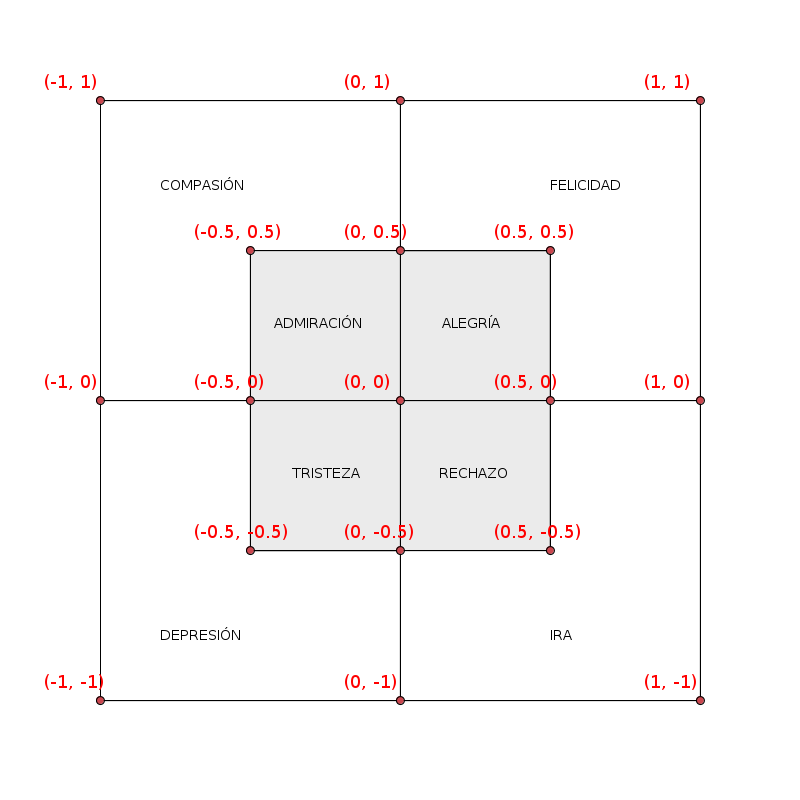
\includegraphics[width=9cm]{ilustraciones/propuesta/modelo-afectivo.png}
\end{ilustracion}

Con respecto a la selección de la emoción por parte del modelo afectivo al recibir un estado emocional,
se tiene el algoritmo de la \refcuadro{algoritmo-modelo-afectivo}, básicamente se
verifica por cada emoción si el punto en el plano proporcionado por el estado emocional
está contenido dentro del polígono de la emoción.

\begin{cuadro}[etiqueta=algoritmo-modelo-afectivo, titulo={Algoritmo del Modelo Afectivo Para la Selección de Una Emoción}]{l}
\toprule
\textbf{Entrada:} estado emocional del agente \\
\midrule
\textbf{Para cada} emoción \textbf{$\in$} conjunto de emociones \textbf{hacer:} \\
~~~~~~\textbf{Si} el punto en \Rcuadrado~del estado emocional está contenido \\
~~~~~~~~~~en el polígono de la emoción \textbf{entonces:} \\
~~~~~~~~~~~~~~\textbf{devolver} emoción \\
~~~~~~\textbf{Fin si} \\
\textbf{Fin para} \\
\bottomrule
\fuentecuadro{1}{\yo}
\end{cuadro}

\subseccion{Base de Conocimiento Conductual}

La Base de Conocimiento Conductual (BCC), es la responsable de la gestión del conocimiento de las
emociones y comportamientos del agente
emocional. Está implementada en el lenguaje de programación lógico \textit{Prolog},
el cual es utilizado de manera extendida para servir como base de conocimiento, debido a que
maneja hechos y reglas, además posee un motor de inferencia que permite extraer
conocimiento a través de cuestionamientos. Este lenguaje ha sido empotrado en Java
por medio del uso de bibliotecas de clases que permiten dicha asociación.

En \textit{Prolog}, un \textit{hecho} es una cláusula que representa una relación entre objetos.
Ejemplo de hecho en \textit{Prolog}: \comillas{\codigoenlinea{capital(francia, paris).}}, la interpretación es:
La capital de Francia es París. En general, la sintaxis es
\comillas{\codigoenlinea{relacion(objeto$_1$, objeto$_2$, ..., objeto$_n$).}}.
La relación se conoce como \textit{predicado} y los objetos como \textit{argumentos}.

Una \textit{regla} consta de dos partes, la cabeza y un cuerpo, ambos unidos por los
símbolos \comillas{:-}, los cuales se leen como \comillas{si} (la cabeza es verdad
si el cuerpo es verdad). La cabeza está compuesta por un solo hecho, y el cuerpo
puede estar constituido por uno o varios hechos, ejemplo:
\comillas{\codigoenlinea{cabeza :- hecho$_1$, hecho$_2$, ..., hecho$_n$.}}.
Ejemplo de regla en \textit{Prolog}: \comillas{\codigoenlinea{hijoDe(A,B) :- padrede(B,A).}},
y su interpretación es: A es hijo de B si B es padre de A.

El conocimiento gestionado por la BCC puede ser de cuatro
tipos, conocimiento sobre \textit{el agente, las emociones,
las reglas de prioridad de los comportamientos y los estímulos}.
Con respecto al agente, en la \refcuadro{conocimiento-sobre-agente}
se observan las cláusulas que definen el conocimiento
en relación a sí mismo y a los demás.

\newpage

\begin{cuadro}[etiqueta=conocimiento-sobre-agente, titulo={Conocimiento Relacionado al Agente en la BCC}]{lp{7cm}}
\toprule
Cláusula & Descripción \\
\midrule
\codigoenlinea{1. yo(agenteEmocional).} & Definición del agente actual. Se utiliza como ejemplo el nombre \codigoenlinea{agenteEmocional} \\ \hline
\codigoenlinea{2. otro(A) :- not yo(A).} & Definición de otro agente. \codigoenlinea{A} es una variable que representa el nombre del agente \\
\bottomrule
\fuentecuadro{2}{\yo}
\end{cuadro}

La \refcuadro{conocimiento-emociones}, muestra los hechos del conocimiento
asociado a los tipos de emociones. La estructura de la regla para definir
un tipo de emoción se compone del predicado, en este caso \codigoenlinea{tipo\_emocion}
y los parámetros: emoción y tipo de emoción.
Dicho conocimiento es definido por MASOES en la \refcuadro{comportamientos-masoes}.

La base de conocimiento conductual también contiene las reglas definidas
por MASOES en las que se asocia un estado emocional a un tipo de comportamiento.
Así, para las reglas de asociación de comportamiento \refpcuadro{reglas-comportamientos-masoes},
se define el conjunto de cláusulas de la
\refcuadro{conocimiento-comportamiento}, donde \codigoenlinea{E} representa la emoción.

\begin{cuadro}[etiqueta=conocimiento-emociones, titulo={Conocimiento Relacionado a las Emociones en la BCC}]{ll}
\toprule
Cláusula & Descripción \\
\midrule
\codigoenlinea{1. tipo\_emocion(admiracion, positiva).} & La admiración es positiva \\ \hline
\codigoenlinea{2. tipo\_emocion(compasion, positiva).} & La compasión es positiva \\ \hline
\codigoenlinea{3. tipo\_emocion(felicidad, positiva).} & La felicidad es positiva \\ \hline
\codigoenlinea{4. tipo\_emocion(alegria, positiva).} & La alegría es positiva \\ \hline
\codigoenlinea{5. tipo\_emocion(rechazo, ligeramente\_negativa).} & El rechazo es ligeramente negativa \\ \hline
\codigoenlinea{6. tipo\_emocion(tristeza, ligeramente\_negativa).} & La tristeza es ligeramente negativa \\ \hline
\codigoenlinea{7. tipo\_emocion(ira, altamente\_negativa).} & La ira es altamente negativa \\ \hline
\codigoenlinea{8. tipo\_emocion(depresion, altamente\_negativa).} & La depresión es altamente negativa \\
\bottomrule
\fuentecuadro{2}{\yo}
\end{cuadro}

\newpage

\begin{cuadro}[etiqueta=conocimiento-comportamiento, titulo={Conocimiento Relacionado a las Comportamientos en la BCC}]{p{6.5cm}p{5cm}}
\toprule
Cláusula & Descripción \\
\midrule
\codigoenlinea{1. prioridad\_comportamiento(E, imitativo) :- tipo\_emocion(E, positiva).} & El comportamiento es imitativo si la emoción \codigoenlinea{E} es positiva \\ \hline
\codigoenlinea{2. prioridad\_comportamiento(E, cognitivo) :- tipo\_emocion(E, ligeramente\_negativa).} & El comportamiento es cognitivo si la emoción \codigoenlinea{E} es ligeramente negativa \\ \hline
\codigoenlinea{3. prioridad\_comportamiento(E, reactivo) :- tipo\_emocion(E, altamente\_negativa).} & El comportamiento es reactivo si la emoción \codigoenlinea{E} es altamente negativa \\
\bottomrule
\fuentecuadro{2}{\yo}
\end{cuadro}

Para agregar estímulos a la BCC, es necesario que
el agente asigne a cada uno de ellos un \textit{Parámetro de Activación ($P_a$)}
y un \textit{Parámetro de Satisfacción ($P_s$)}, estos valores
incrementarán o decrementaran la activación y satisfacción del agente.
La estructura para definir un estímulo se compone del predicado
\codigoenlinea{estimulo} y los argumentos:
nombre del agente, nombre del estímulo, $P_a$ y $P_s$.
En el \refcuadro{definicion-eventos}, se muestran algunos ejemplos de definiciones de estímulos.

\begin{cuadro}[etiqueta=definicion-eventos, titulo={Ejemplos de Conocimiento de Estímulos en la BCC}]{lp{6cm}}
\toprule
Cláusula & Descripción \\
\midrule
\codigoenlinea{1. estimulo(A, saludar, 0.01, 0.01) :- otro(A).} & Para el agente \codigoenlinea{A} el estímulo saludar aumentará la activación en 0.01 y la satisfacción en 0.01 si el estímulo fue enviado por otro agente \\ \hline
\codigoenlinea{2. estimulo(A, despertar, 0.02, -0.1) :- yo(A).} & Para el agente \codigoenlinea{A} el estímulo despertar aumentará la activación en 0.02 y disminuirá la satisfacción en 0.1 si el evento fue generado por el mismo agente \\
\bottomrule
\fuentecuadro{2}{\yo}
\end{cuadro}

\subseccion{Configurador Emocional}

Este elemento tiene la responsabilidad de evaluar los estímulos y actualizar
la emoción del agente. Para esto se definen las siguientes ecuaciones de actualización
para la activación y la satisfacción:

\begin{ecuacion}{actualizacion-activacion}
  A'(ag_i) = A_i + P_A
\end{ecuacion}

Donde $A'(ag_i)$ representa el nuevo valor de activación del agente $ag_i$,
$A_i$ es la activación actual y $P_A$ se define como el parámetro de activación
obtenido de la BCC, y esta comprendido en el intevalo: $-1 \leq P_A \leq 1$.

\begin{ecuacion}{actualizacion-satisfaccion}
  S'(ag_i) = S_i + P_S
\end{ecuacion}

Donde $S'(ag_i)$ representa el nuevo valor de satisfacción del agente $ag_i$,
$S_i$ es la satisfacción actual y $P_S$ es el parámetro de
satisfacción obtenido de la BCC, y se encuentra en el intervalo: $-1 \leq P_S \leq 1$.

Para obtener el estímulo, el configurador emocional hará un
cuestionamiento a la BCC, para ello se consulta
un hecho utilizando los símbolos \comillas{?-} con el siguiente formato en lenguaje \textit{Prolog}:

{
\ttfamily \fontsize{10pt}{10pt}\selectfont
\noindent ?- estimulo(nombreAgente, nombreEstimulo, PA, PS).
}

Las variables \comillas{\codigoenlinea{PA}} y \comillas{\codigoenlinea{PS}},
son las incógnitas a conocer.
En el siguiente ejemplo \refpcuadro{ejemplo-consulta-activacion}, se puede observar
como se consulta el evento saludar en la BCC y el formato de la respuesta de ésta.
El algoritmo de actualización del estado emocional del agente se muestra en la
\refcuadro{algoritmo-configurador-emocional}.

\newpage

\begin{cuadro}[etiqueta=ejemplo-consulta-activacion, titulo={Ejemplo de Consulta a la BCC de un Estímulo}]{ll}
\toprule
Cláusula & Descripción \\
\midrule
\codigoenlinea{1. yo(agenteA).} & Definición del agente actual \\ \hline
\codigoenlinea{2. otro(A) :- not yo(A).} & Regla que define a otros agentes \\ \hline
\codigoenlinea{3. estimulo(A, saludar, 0.01, 0.01) :- otro(A).} & Definición del estímulo saludar \\ \hline
\codigoenlinea{4. ?- estimulo(agenteB, saludar, PA, PS).} & Consulta del estímulo saludar enviado por el \codigoenlinea{agenteB} \\ \hline
\codigoenlinea{5. PA = 0.01} & Respuesta obtenida sobre el parámetro de activación \\ \hline
\codigoenlinea{6. PS = 0.01} & Respuesta obtenida sobre el parámetro de satisfacción \\
\bottomrule
\fuentecuadro{2}{\yo}
\end{cuadro}

\begin{cuadro}[etiqueta=algoritmo-configurador-emocional, titulo={Algoritmo del Configurador Emocional Para la Actualización del Estado Emocional del Agente}]{l}
\toprule
\textbf{Entrada:} estímulo y BCC \\
\midrule
Consultar en la BCC si el estímulo existe \\
\textbf{Si} existe conocimiento del estímulo \textbf{entonces:} \\
~~~~~PA  $\leftarrow$ obtener PA desde BCC \\
~~~~~PS  $\leftarrow$ obtener PS desde BCC \\
~~~~~Activación $\leftarrow$ Activación + PA \\
~~~~~Satisfacción $\leftarrow$ Satisfacción + PS \\
~~~~~Estado Emocional $\leftarrow$ Crear nuevo Estado Emocional a partir de los nuevos \\
~~~~~~~~~~~~~~~~~~~~~~~~~~~~~~~~~~~valores de Activación y Satisfacción \\
~~~~~Emoción $\leftarrow$ Consultar emoción en Modelo Afectivo a partir del nuevo Estado Emocional \\
\textbf{Fin si} \\
\bottomrule
\fuentecuadro{1}{\yo}
\end{cuadro}

\subseccion{Manejador de Comportamiento}

El Manejador de Comportamiento se encarga de actualizar la prioridad del comportamiento a ejecutar
por el agente, se basa en la reglas de prioridad definidas en MASOES \refpcuadro{reglas-comportamientos-masoes}
y el estado emocional actual.

Tiene como entrada la emoción dada por el configurador emocional.
Para obtener el tipo de comportamiento asociado a la emoción,
este componente consulta la BCC, con el siguiente formato en lenguaje \textit{Prolog}:

{
\ttfamily \fontsize{10pt}{10pt}\selectfont
\noindent ?- prioridad\_comportamiento(nombreEmocion, TIPO).
}

Este cuestionamieto retorna el valor de la variable \comillas{\codigoenlinea{TIPO}},
que puede ser \comillas{\codigoenlinea{imitativo}},
\comillas{\codigoenlinea{cognitivo}} y \comillas{\codigoenlinea{reactivo}}.

El siguiente ejemplo \refpcuadro{ejemplo-consulta-comportamiento} muestra el
resultado de preguntarle a la BCC el tipo de comportamiento asociado a la emoción
admiración.

\begin{cuadro}[etiqueta=ejemplo-consulta-comportamiento, titulo={Ejemplo de Consulta a la BCC del Tipo de Comportamiento Asociado a Una Emoción}]{p{7cm}p{5cm}}
\toprule
Cláusula & Descripción \\
\midrule
\codigoenlinea{1. tipo\_emocion(admiracion, positiva).} & Define que la Admiración es una emoción positiva \\ \hline
\codigoenlinea{2. prioridad\_comportamiento(E, imitativo) :- tipo\_emocion(E, positiva).} & Regla que define el comportamiento imitativo para una emoción \codigoenlinea{E} \\ \hline
\codigoenlinea{3. ?- prioridad\_comportamiento(admiracion, TIPO).} & Se consulta a la BCC cual es el comportamiento asociado a la admiración \\ \hline
\codigoenlinea{4. TIPO = imitativo} & Respuesta obtenida \\
\bottomrule
\fuentecuadro{2}{\yo}
\end{cuadro}

Para la actualización de la prioridad del comportamiento se implementó el algoritmo
de la \refcuadro{algoritmo-manejador-comportamiento}.

\begin{cuadro}[etiqueta=algoritmo-manejador-comportamiento, titulo={Algoritmo del Manejador de Comportamiento Para la Actualización de la Prioridad de Comportamiento}]{l}
\toprule
\textbf{Entrada:} emoción provista por el configurador emocional \\
\midrule
Consultar en la BCC la prioridad del comportamiento \\
\textbf{Si} existe comportamiento asociado a la emoción \textbf{entonces:} \\
~~~~~Comportamiento  $\leftarrow$ obtener comportamiento desde BCC \\
\textbf{Fin si} \\
\bottomrule
\fuentecuadro{1}{\yo}
\end{cuadro}

\subseccion{Procesamiento de Estímulo}

En el siguiente diagrama de flujo \refpilustracion{procesamiento-estimulo},
se expone el procedimiento implementado en la propuesta para realizar la gestión del estímulo
desde que se genera o recibe hasta que se actualiza el comportamiento del agente.

\begin{ilustracion}[fuente=\yo, etiqueta=procesamiento-estimulo, titulo={Flujo de Procesamiento de Estímulo}]
\includegraphics[width=12cm]{ilustraciones/diagramas-puml/procesamiento-estimulo.png}
\end{ilustracion}

El flujo puede iniciarse al recibir del entorno u otro agente un estímulo,
o al ser generado internamente, posterior a eso, el agente delega la responsabilidad a su componente
conductual, cuando el estímulo no es conocido,
el componente conductual detiene su ejecución, el flujo termina y se mantiene la emoción y comportamiento actual,
si el estímulo es conocido el componente consultará en su BCC
los parámetros de activación y satisfacción y actualizará la emoción.
Luego, el manejador de comportamiento
consulta la BCC para obtener
la prioridad asociada a la nueva emoción
que exhibe el agente, y actualiza la prioridad del comportamiento (reactivo, cognitivo o imitativo).
Finalmente, el agente modifica su comportamiento.

\seccion{Aspectos Propuestos a Nivel Colectivo}

\subseccion{Cálculo de la Emoción Social}

\cite{rincon2015} proponen un modelo de emoción social basado en el modelo
psicológico de estados emocionales PAD \eningles{Pleasure, Arousal and
Dominance}. PAD es un modelo que representa el estado emocional de un agente en
tres dimensiones, placer, excitación y dominio.
Este modelo utiliza las
emociones individuales de cada entidad de un grupo de agentes, para calcular la
\textit{emoción social}, la cual se compone de tres valores: \textit{emoción central,
distancia máxima con respecto a la emoción central y dispersión emocional}.
Basado en lo definido por \cite{rincon2015},
a continuación se expone la propuesta para el cálculo de la \textit{emoción social}:

Como está definido en MASOES \citep{perozo2011}, la emoción individual es un
vector en \Rcuadrado~y esta representada por la
\refecuacion{emocion-individual}.

\begin{ecuacion}{emocion-individual}
  E(ag_i) = (A_i , S_i)
\end{ecuacion}

Donde $ag_i$ es un agente, $A_i$ es la activación del agente y $S_i$ es la
satisfacción del agente.

La \textbf{Emoción Social} está representada por un conjunto de tres valores
\refpecuacion{emocion-social}.

\begin{ecuacion}{emocion-social}
  ES(Ag) = \{EC(Ag), m(Ag), \sigma(Ag)\}
\end{ecuacion}

Donde $Ag$ representa al grupo de agentes en estudio, $EC(Ag)$ se refiere a la
emoción central exhibida por el grupo de agentes, $m(Ag)$ es el estado emocional
más alejado de la $EC$, $\sigma(Ag)$ representa la dispersión emocional entorno
a la $EC$.

La \textbf{Emoción Central} dada por la \refecuacion{emocion-central}, se define
como la emoción promedio \refpecuacion{emocion-central-promedios} que exhibe un
grupo de agentes $Ag$, este concepto se introduce debido a que dos grupos de agentes
pueden tener la misma $EC$ para agentes muy cercanos o muy alejados de ella,
de esta manera se puede hacer una mejor interpretación de la $EC$.

\begin{ecuacion}{emocion-central}
  EC(Ag) = (\bar A(Ag), \bar S(Ag))
\end{ecuacion}

Donde $Ag$ representa al grupo de agentes en estudio, $\bar A$ es el promedio
de activación y $\bar S$ el promedio de satisfacción del grupo en estudio.

\begin{ecuacion}{emocion-central-promedios}
  \begin{split}
    \bar A(Ag)=\frac{\sum_{i=1}^n A_i}{n}, \forall ag_i \in Ag \\
    \bar S(Ag)=\frac{\sum_{i=1}^n S_i}{n}, \forall ag_i \in Ag
    \end{split}
\end{ecuacion}

Donde $Ag$ representa al grupo de agentes en estudio, $A_i$ es la activación y $S_i$ la satisfacción del agente $i$, para $1 \leq i \leq n$.

La \textbf{Distancia Máxima} con respecto a la $EC$ \refpecuacion{distancia-maxima},
permite saber si existen agentes con estados emocionales muy lejanos o cercanos
a la emoción central. Se define como la distancia máxima euclidiana
\refpecuacion{distancia-maxima-especifica} con respecto a la emoción central.

\begin{ecuacion}{distancia-maxima}
  m(Ag) = (m_A(Ag), m_S(Ag))
\end{ecuacion}

Donde $Ag$ representa al grupo de agentes en estudio, $m_A(Ag)$ es
la activación más alejada (máxima activación) y $m_S(Ag)$ es la satisfacción más
alejada (máxima satisfacción).

\begin{ecuacion}{distancia-maxima-especifica}
  \begin{split}
  m_A(Ag) = max\left(\sqrt{(A_i - \bar A(Ag))^2}\right), \forall ag_i \in Ag \\
  m_S(Ag) = max\left(\sqrt{(S_i - \bar S(Ag))^2}\right), \forall ag_i \in Ag
  \end{split}
\end{ecuacion}

Donde $Ag$ es el grupo de agentes, $A_i$ es la activación y $S_i(Ag)$ la satisfacción del agente $ag_i$,
 $\bar A$ es el promedio de activación y $\bar S(Ag)$ el promedio de satisfacción del grupo en estudio.

Para una mejor comprensión de la diversidad de emociones en el grupo de agentes,
surge la \textbf{Dispersión Emocional} entorno a la $EC$ representada por la
\refecuacion{dispersion-emocional} y se define como la desviación estándar con
respecto a la emoción central \refpecuacion{dispersion-emocional-especifica}.

\begin{ecuacion}{dispersion-emocional}
  \sigma(Ag) = (\sigma_A(Ag), \sigma_S(Ag))
\end{ecuacion}

Donde $\sigma_A(Ag)$ es la desviación estándar de la activación y
$\sigma_S(Ag)$ es la desviación estándar de la satisfacción del grupo
de agentes $Ag$.

\begin{ecuacion}{dispersion-emocional-especifica}
  \begin{split}
  \sigma_A(Ag) = \sqrt{\frac{\sum_{i=1}^n(A_i - \bar A(Ag))^2}{n}},  \forall ag_i \in Ag \\
  \sigma_S(Ag) = \sqrt{\frac{\sum_{i=1}^n(S_i - \bar S(Ag))^2}{n}},  \forall ag_i \in Ag
  \end{split}
\end{ecuacion}

Donde $Ag$ es el grupo de agentes, $A_i$ es la activación y $S_i$ la satisfacción del agente $ag_i$,
para $1 \leq i \leq n$, $\bar A(Ag)$ es el promedio de activación y $\bar S(Ag)$
el promedio de satisfacción del grupo en estudio.

Si $\sigma(Ag) \gg 0$, el grupo tiene una alta dispersión emocional, es decir, los
miembros del grupo tienen diferentes estados emocionales (muy heterogéneos).

Si $\sigma (Ag) \cong 0$, el
grupo tiene una dispersión emocional baja, esto significa que los individuos
tienen estados emocionales similares (muy homogéneos).

\seccion{Herramienta Computacional Desarrollada}

El código fuente desarrollado para este trabajo de investigación se encuentra
disponible bajo la licencia GPL \eningles{General Public License}, y se puede
acceder a través de la dirección \url{http://bit.ly/UnaImplementacionDeMASOES}.
Se utilizó \codigoenlinea{Java} como lenguaje de programación en su versión 8.

Las librerías empleadas para el desarrollo de la herramienta computacional se nombran a continuación:

\begin{vinetas}
    \item \codigoenlinea{JADE 4.4.0} como plataforma para el desarrollo de los
    agentes de software.
    \item \codigoenlinea{JTS 1.13} para los cálculos geométricos asociados al
    modelo afectivo.
    \item \codigoenlinea{Miglayout 5.0} para el desarrollo de las interfaces
    de usuario.
    \item \codigoenlinea{TuProlog 3.2} como intérprete del lenguaje Prolog dentro de Java.
    \item \codigoenlinea{jFreeChart 1.0.19} para la creación de gráficos en tiempo real.
    \item \codigoenlinea{jUnit 4.12}, \codigoenlinea{Mockito 1.10.19} y \codigoenlinea{PowerMock 1.6.5}
    en combinación para pruebas unitarias y funcionales.
    \item \codigoenlinea{commons-cli 1.3.1} como interpretador de comandos, utilizado
    en los agentes emocionales para extraer argumentos.
    \item \codigoenlinea{jackson 2.9.0} para exportar e importar una configuración a través de archivos de texto.
\end{vinetas}

\espaciodoble

La herramienta proporciona diversos comandos que permiten llevar a cabo
diferentes tareas, se listan en la \refcuadro{comandos-para-ejecuacion}:

\begin{cuadro}[etiqueta=comandos-para-ejecuacion, titulo={Lista de Comandos Para la Ejecución de la Herramienta}]{l|p{8cm}}
\toprule
Comando & Descripción \\
\midrule
\codigoenlinea{make help} & Muestra la ayuda \\
\codigoenlinea{make unit-test} & Ejecuta las pruebas unitarias \\
\codigoenlinea{make fuctional-test} & Ejecuta las pruebas funcionales \\
\codigoenlinea{make test} & Ejecuta las pruebas unitarias y funcionales a la vez \\
\codigoenlinea{make run} & Levanta la plataforma sin agentes instanciados \\
\codigoenlinea{make simulation} & Levanta la plataforma con los agentes necesarios para llevar a cabo una simulación \\
\bottomrule
\fuentecuadro{2}{\yo}
\end{cuadro}

\subseccion{Configuraciones de JADE Para la Ejecución de la Plataforma}

Se proporciona el archivo \codigoenlinea{jade.properties} en la ruta del proyecto con la finalidad
de registrar las configuraciones necesarias para la ejecución de la plataforma,
dichos valores se mustran en la \refcuadro{configuracion-jade}:

\newpage

\begin{cuadro}[etiqueta=configuracion-jade, titulo={Lista de Configuraciones de JADE Utilizadas Para la Ejecución de la Herramienta Computacional}]{l|cp{6cm}}
\toprule
Configuración & Valor por Omisión & Descripción \\
\midrule
\codigoenlinea{gui} & \codigoenlinea{true} & Le indica a JADE si la ejecución será en modo interfaz de usuario (\codigoenlinea{true}) o en modo servidor (\codigoenlinea{false}). \\
\codigoenlinea{port} & \codigoenlinea{1099} & Se refiere al puerto que utilizara JADE para conectar diferentes contenedores de agentes localmente o a través de una red. El protocolo usado es JICP \eningles{JADE Inter Container Protocol}  \\
\codigoenlinea{jade\_mtp\_http\_port} & \codigoenlinea{7778} & Puerto utilizado por JADE para la transmisión de mensajes de agentes localmente o a través de una red. El protocolo usado es IMTP \eningles{Instant Message Transfer Protocol}  \\
\codigoenlinea{jade\_domain\_df\_autocleanup} & \codigoenlinea{true} & Le indica al agente DF de JADE que debe limpiar los servicios de un agente en caso de que sea eliminado (\codigoenlinea{true}), de esta manera se asegura que no haya información inconsistente en el DF. \\
\codigoenlinea{platform-id} & \codigoenlinea{masoes} & Debido a que se puede instanciar diferentes plataformas localmente o en una red, es necesario asignar un identificador único a cada una. \\
\bottomrule
\fuentecuadro{3}{\yo}
\end{cuadro}

\subseccion{Agentes del Entorno Propuestos Para MASOES}

El entorno está constituido por diversos agentes emocionales y no emocionales,
con la finalidad de cumplir diversos roles necesarios para el funcionamiento de
la implementación, por esta razón se proponen los siguientes agentes.

\subsubseccion{Agente Emocional}

En la \refseccion{propuesta-nivel-individual} se vió el diseño del agente emocional a nivel individual.
A continuación se listan los argumentos (opcionales) que pueden ser enviados al agente al momento de ser
instanciado en la plataforma:

\begin{cuadro}[etiqueta=argumentos-agente-emocional, titulo={Lista de Argumentos Para el Agente Emocional}]{l|p{8cm}}
\toprule
Argumento & Descripción \\
\midrule
\codigoenlinea{a} & \textbf{Activación:} Asigna la activación inicial del agente emocional \\
\codigoenlinea{s} & \textbf{Satisfacción:} Asigna la satisfacción inicial del agente emocional\\
\codigoenlinea{k} & \textbf{Importar Conocimiento:} Permite importar al agente conocimiento desde una cadena de caracteres \\
\codigoenlinea{kp} & \textbf{Importar Conocimiento Desde Archivo de Texto:} Ruta del archivo de texto con el conocimiento sobre los estímulos para el agente \\
\bottomrule
\fuentecuadro{2}{\yo}
\end{cuadro}

\subsubseccion{Agente Notificador}

El Agente Notificador tiene como responsabilidad notificar a todos los agentes de
las acciones, objetos o eventos que van aconteciendo en el sistema.
Se desarrolló para este trabajo de investigación con el objetivo de comunicar una
acción, objeto o evento al resto de agentes del campo de acción.

En la \refilustracion{ontologia-masoes-notificar-estimulo},
se observan las entidades de la ontología propuesta para MASOES, que permiten la interacción
con este agente. Cualquier agente puede enviar una notificación de tipo objeto, acción o evento,
cuando la acción se haya completado el agente notificador enviará una respuesta tipo \textit{Done},
esta entidad es provista por JADE e indica que la solicitud fue realizada satisfactoriamente.

\begin{ilustracion}[fuente=\yo, etiqueta=ontologia-masoes-notificar-estimulo, titulo={Ontología para MASOES, Acciones de Notificación}]
\includegraphics[width=11cm]{ilustraciones/diagramas-puml/ontologia-masoes-notificar-estimulo.png}
\end{ilustracion}

A través del diagrama de la \refilustracion{flujo-agente-notificador}, se explica el procedimiento
que realiza este agente para comunicar un estímulo. En primer lugar, recibe una petición de acción,
luego solicita la lista de agentes emocionales al DF, por último, envía un estímulo
a cada agente de la lista y responde con un objeto \textit{Done} al agente emisor.

\begin{ilustracion}[fuente=\yo, etiqueta=flujo-agente-notificador, titulo={Comunicación con el Agente Notificador}]
\includegraphics[width=11cm]{ilustraciones/diagramas-puml/flujo-agente-notificador.png}
\end{ilustracion}

\subsubseccion{Agente Para el Cálculo de la Emoción Social}

\label{agente-calculador-emocion-social}

Se propone un agente
que encapsula el cálculo de la emoción social
propuesta en este trabajo. Se incluyen entidades en la ontología de MASOES que permiten
la interacción con otros agentes.
Para que un agente pueda conocer la emoción social
debe enviar una solicitud de tipo \textit{ConsultarEmocionSocial},
el agente calculador enviará una respuesta de tipo \textit{EmocionSocial}
con los valores de la emoción central, dispersión emocional
y distancia máxima \refpilustracion{ontologia-masoes-emocion-social}.

En el diagrama de la \refilustracion{flujo-agente-emocion-social}, se ilustra el procedimiento
de comunicación entre agentes, se incluye las entidades ontológicas usadas en dicha comunicación.
Este agente debe consultar al DF el listado de agentes emocionales en la plataforma,
posteriormente, solicita el estado emocional a cada uno de ellos y procede a calcular la emoción
social.

\begin{ilustracion}[fuente=\yo, etiqueta=ontologia-masoes-emocion-social, titulo={Ontología para MASOES, Acción Consultar Emoción Social}]
\includegraphics[width=12cm]{ilustraciones/diagramas-puml/ontologia-masoes-emocion-social.png}
\end{ilustracion}

\begin{ilustracion}[fuente=\yo, etiqueta=flujo-agente-emocion-social, titulo={Comunicación con el Agente Calculador de Emoción Social}]
\includegraphics[width=13cm]{ilustraciones/diagramas-puml/flujo-agente-emocion-social.png}
\end{ilustracion}

\subsubseccion{Agente Interfaz: Estado del Agente}

Es posible observar el estado emocional de un agente en tiempo de ejecución a través de la interfaz
\comillas{Estado del Agente} \refpilustracion{interfaz-estado-agente}.
Esta incluye el gráfico del modelo afectivo de MASOES y la información correspondiente al estado emocional.
Se debe crear en la plataforma un agente de tipo: \codigoenlinea{gui.agentstate.AgentStateGuiAgent},
dandole como argumento el
nombre del agente el cual se desea observar su estado emocional.

\begin{ilustracion}[fuente=\yo, etiqueta=interfaz-estado-agente, titulo={Interfaz Para Observar el Estado Emocional Dado un Agente}]
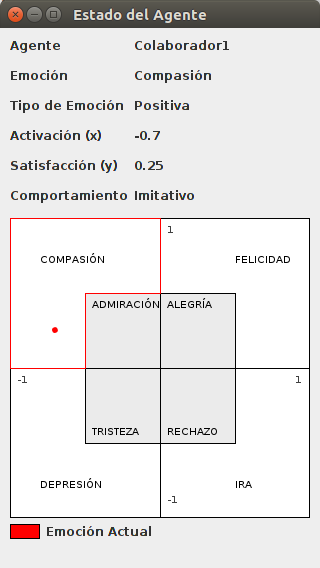
\includegraphics[width=7cm]{ilustraciones/interfaces/estado-agente.png}
\end{ilustracion}

\subsubseccion{Agente Interfaz: Emoción Social}

Se proporciona la interfaz \comillas{Emoción Social} para poder observar la emoción social actual
en tiempo de ejecución \refpilustracion{interfaz-emocion-social}, dicha interfaz se conectara automáticamente con el agente descrito en la \refseccion{agente-calculador-emocion-social}.
Esta incluye el gráfico del modelo afectivo de MASOES y la información correspondiente a
la emoción social. Se debe instanciar en la plataforma un agente de tipo: \codigoenlinea{gui.socialemotion.SocialEmotionGuiAgent}.

\begin{ilustracion}[fuente=\yo, etiqueta=interfaz-emocion-social, titulo={Interfaz Para Observar la Emoción Social del Grupo de Agentes}]
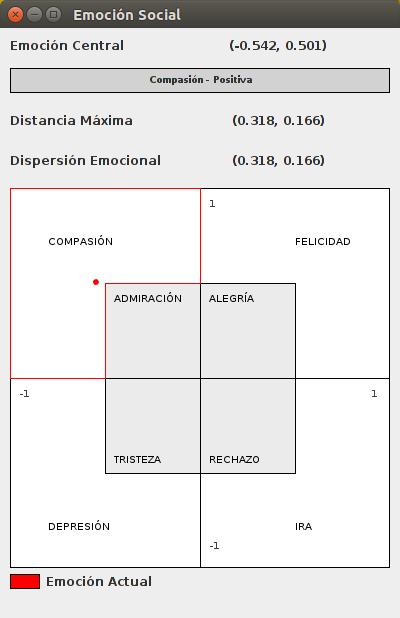
\includegraphics[width=8cm]{ilustraciones/interfaces/emocion-social.png}
\end{ilustracion}

\subsubseccion{Agente Interfaz: Para el Envío de Mensajes}

En la \refilustracion{envio-de-mensajes}
se muestra la ventana para envío de mensajes manualmente, es desarrollada con la finalidad de observar
los mensajes que se envían y reciben en una conversación entre dos agentes.
Se instancia a través de la clase: \codigoenlinea{gui.requester.RequesterGuiAgent}.

\begin{ilustracion}[fuente=\yo, etiqueta=envio-de-mensajes, titulo={Interfaz Para Envío de Mensajes Manualmente}]
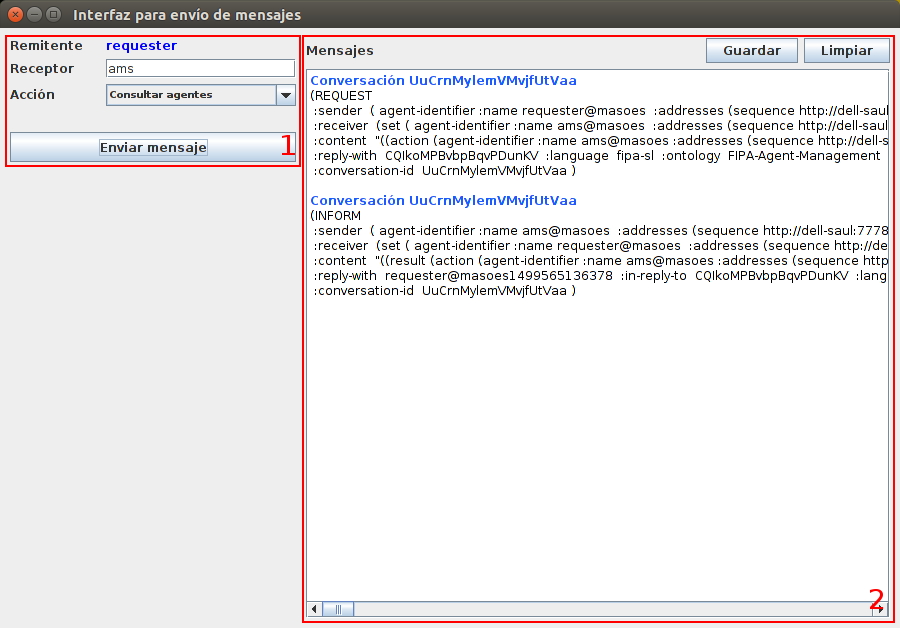
\includegraphics[width=14cm]{ilustraciones/interfaces/interfaz-para-envio-de-mensajes-recuadros.png}
\end{ilustracion}

Dicha interfaz se compone de dos secciones:

\begin{enumeracion}
	\item \textbf{Acciones:} Permite configurar el mensaje que se enviará, contiene un conjunto de mensajes o acciones
  preconfiguradas.
	\item \textbf{Mensajes}: Muestra los mensajes enviados y recibidos, además, proporciona dos botones
  que permiten guardar los mensajes en un archivo de texto y limpiar la ventana.
\end{enumeracion}

\subsubseccion{Agente Interfaz: Simulador}

La interfaz de usuario denominada simulador \refpilustracion{simulador},
permite definir los tipos de agentes y estímulos para un determinado caso de estudio, además
provee la posibilidad de establecer una configuración inicial para cada agente
(como el estado emocional y estímulos asociados a dicho agente) e instancia los agentes en la plataforma.

\begin{ilustracion}[fuente=\yo, etiqueta=simulador, titulo={Interfaz Para la Configuración de Simulaciones}]
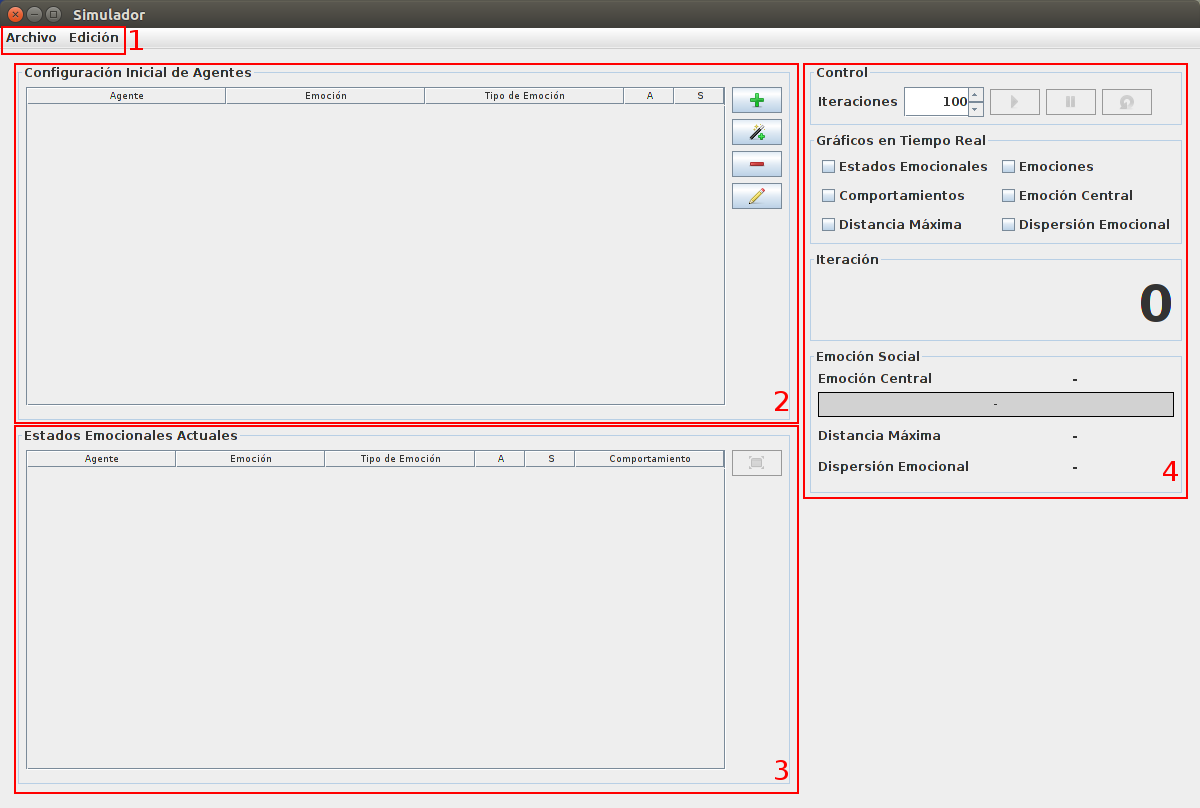
\includegraphics[width=14cm]{ilustraciones/interfaces/simulador-recuadros.png}
\end{ilustracion}

Las secciones que la componen son:

\begin{enumeracion}
	\item \textbf{Barra de Menú:} En el menú \textit{Archivo} se proveen las opciones exportar e importar configuración.
  A través del menú \textit{Edición} se pueden definir los tipos de agentes y estímulos necesarios para la simulación.
  \item \textbf{Configuración Inicial de Agentes:} permite establecer los parámetres de cada agente en la simulación.
  \item \textbf{Estados Emocionales Actuales:} esta tabla muestra los estados emocionales del grupo de agentes en tiempo de ejecución de la simulación.
  \item \textbf{Información General de la Simulación:} en esta sección se puede controlar la simulación,
  activar o desactivar gráficos en tiempo real, asignar el número de iteraciones deseados y ver la iteración y
  la emoción social actual.
\end{enumeracion}

\subseccion{Servicios Expuestos en Agente DF}

Para que los agentes dentro de la plataforma JADE descubran
las acciones que pueden llevar a cabo los demás, se publican los siguientes servicios \refpcuadro{servicios-df}.
Cada agente al ser creado en JADE notificará sus servicios al DF,
es importante destacar que dichos servicios concuerdan con las acciones
en la ontología propuesta para MASOES.

\begin{cuadro}[etiqueta=servicios-df, titulo={Lista de Servicios Expuestos en el Agente DF para la Ontología Propuesta para MASOES}]{l|l}
\toprule
Agente & Servicio \\
\midrule
Agente Emocional & \textit{EvaluarEstimulo} \\
& \textit{ConsultarEstadoEmocional} \\
Agente Notificador  & \textit{NotificarObjeto} \\
& \textit{NotificarAccion} \\
& \textit{NotificarEvento} \\
Agente Calculador de Emoción Social & \textit{ConsultarEmocionSocial} \\
\bottomrule
\fuentecuadro{2}{\yo}
\end{cuadro}
